	% !TeX spellcheck = fr_FR
	
	Comme mentionné dans l'introduction, la principale contribution de cette thèse est d'étudier l'impact de la relation de dominance sur les stratégies de négociation dans le cadre de négociation collaborative entre un agent conversationnel et un utilisateur humain. 
	Pour ce faire, nous devons construire un modèle de négociation qui permettent aux négociateurs de présenter leurs stratégies de négociation. 
	
	Dans ce chapitre, nous présentons notre modèle de négociation collaborative sur lequel sera construit notre modèle de décision basé sur la dominance. 
	
	Afin de définir un système de dialogue dans lequel la relation de dominance régit le choix du prochain énoncé, nous avons d'abord enregistré des dialogues de négociation entre deux personnes afin d'observer leurs comportements dans un cadre de dialogue social de type "négociation collaborative". Nous avons annotés et analysé les dialogues. Cette étude nous a livré un ensemble de comportements  que nous présenterons dans la première section de ce chapitre. 
	
	Les informations collectées grâce l'observation des comportements humains nous a guidés dans la conception de notre modèle de négociation.
	
	
	
	Dans la seconde section, nous présenterons le domaine de négociation utilisé. Dans le cadre de cette thèse, nous nous basons sur les modèles de négociations multi-critères largement utilisé dans la mise en œuvre de systèmes de négociations automatiques. 
	
	La troisième section présentera notre modèle de communication basé sur des actes de dialogues. En effet, nous nous sommes réapproprié les actes de dialogue de \cite{grosz1986attention} pour la négociation collaborative.
	
	
	 \section{Collecte de données}
		 Afin de définir un système de dialogue social dans lequel la relation de dominance régit le choix du prochain énoncé, nous avons d'abord effectuer une étude dans laquelle nous avons analyser les comportements de deux interlocuteurs dans un cadre de dialogue social de type "négociation collaborative". 
		Le but du dialogue est de trouver un restaurant où dîner avec son interlocuteur. De plus, les interlocuteurs n'avaient pas de connaissances prérequis sur les préférences de leur interlocuteur.
		
		Une fois le dialogue enregistré, nous les avons annoté et analyser la structure du dialogue en suivant la théorie de \emph{Grosz et Sidner} \cite{sidner1994artificial} qui stipule que la structure du dialogue est composée de trois éléments à savoir la structure linguistique, la structure intentionnelle et enfin l'état attentionnel.	
		Nous présenterons dans ce qui suit la procédure de l'analyse ainsi que les résultats obtenus. 
		
		\subsection{Analyse de la structure de dialogue}  
			La théorie présenté par \emph{Grosz et Sidner} propose que la structure d'un dialogue orienté tâche est constituée de trois éléments, chacun agissant sur un aspect du dialogue. 
			
			D'abord, \emph{la structure linguistique} a pour but de décomposer le dialogue en une séquence de segments de dialogue appelé (\textit{DS: discourse segment }) de tel sorte que chaque segment est composé d'un ensemble de sous-segments et d'une séquence d'énoncés appartenant uniquement au segment(n'appartient pas a un sous segment). De plus, les énoncés au sein d'un même segment contribuent à un même but. Cette décomposition est non strict du fait qu'il est difficile de trouver des indices de segmentation. Des exemples d'indices proposés sont l'intention communicative commune à chaque DS, des expressions  linguistiques comme l'utilisation de termes "d'abord, finalement, $\ldots$". Des indices plus subtiles tels que le changement d'intonation, le temps de pause peuvent aussi être utilisés.
			
	%	\subsection{Structure intentionnelle}
			Ensuite vient \emph{la structure intentionnelle}. En effet, un interlocuteur s'engage dans un dialogue poussé par une ou plusieurs intentions internes qu'on nomme \emph{DP: discourse purpose}. De plus, pour chaque \emph{DS}, nous pouvons isolé un but spécifique noté \emph{DSP: Discourse segment purpose}. Le but est d'analyser comment les\emph{ DSPs} participent à la satisfaction du \emph{DS} initial. En outre, cette structure comprend l'analyse des relations entre les différents \emph{DSPs}. Deux relations ont été identifiées, \emph{dominance} et \emph{satisfaction-precedence}. Si la satisfaction de l'intention d'un \emph{DSP1} participe a la satisfaction de celle d'un \emph{DSP2}, alors le \emph{DSP1} \textbf{contribue} au \emph{DSP2}. Par opposition le \emph{DSP2} \textbf{domine} le \emph{DSP1}.
	
			
			Finalement, \emph{l'état attentionnel} s'intéresse à l'abstraction de l'attention des participants au fur et à mesure que leur dialogue avance \cite{sidner1994artificial}. Il est défini avec une pile dynamique \emph{focus stack} qui enregistre les objets, propriétés et les intentions saillantes  à un moment donné dans le dialogue. Le processus de manipulation des espaces dans le dialogue sur la pile attentionnelle (\emph{focus stack}). Cette pile est aussi utilisé pour faciliter l'identification des relations entre les différents \emph{DSPs}
			
%			% Dynamic stack that records salient objects, properties and relations Focusing – process of manipulating focus spaces on attentional (focus) stack
%			 Focus space: les entités saillantes du dilaogue

		 \subsection{Exemple de l'analyse}
			 Nous présentons dans cette section un exemple de l'analyse dite en DSP que nous avons effectué sur un dialogue préalablement enregistré. Le texte a été édité afin d'améliorer son intelligibilité en supprimant les pauses et des mots tels que "hmm, oué $\ldots$".
			 
			 D'abord, nous nous sommes intéressés à la structure linguistique. En effet, nous avons extrait les actes de dialogues de chaque tour de dialogue, que nous avons ensuite regroupé en \emph{DS}. 
			 
			 La seconde étape consistait à analyser le but ou l'intention caché derrière chaque \emph{DS}. Par conséquent, nous avons formulé les \emph{DSPs} comme présenté dans l'exemple ci-dessus. L'état attentionnel nous a aidé à la construction des différents \emph{DS} et a formuler les intentions pour chaque \emph{DSP}	
			
			
			\begin{figure}
				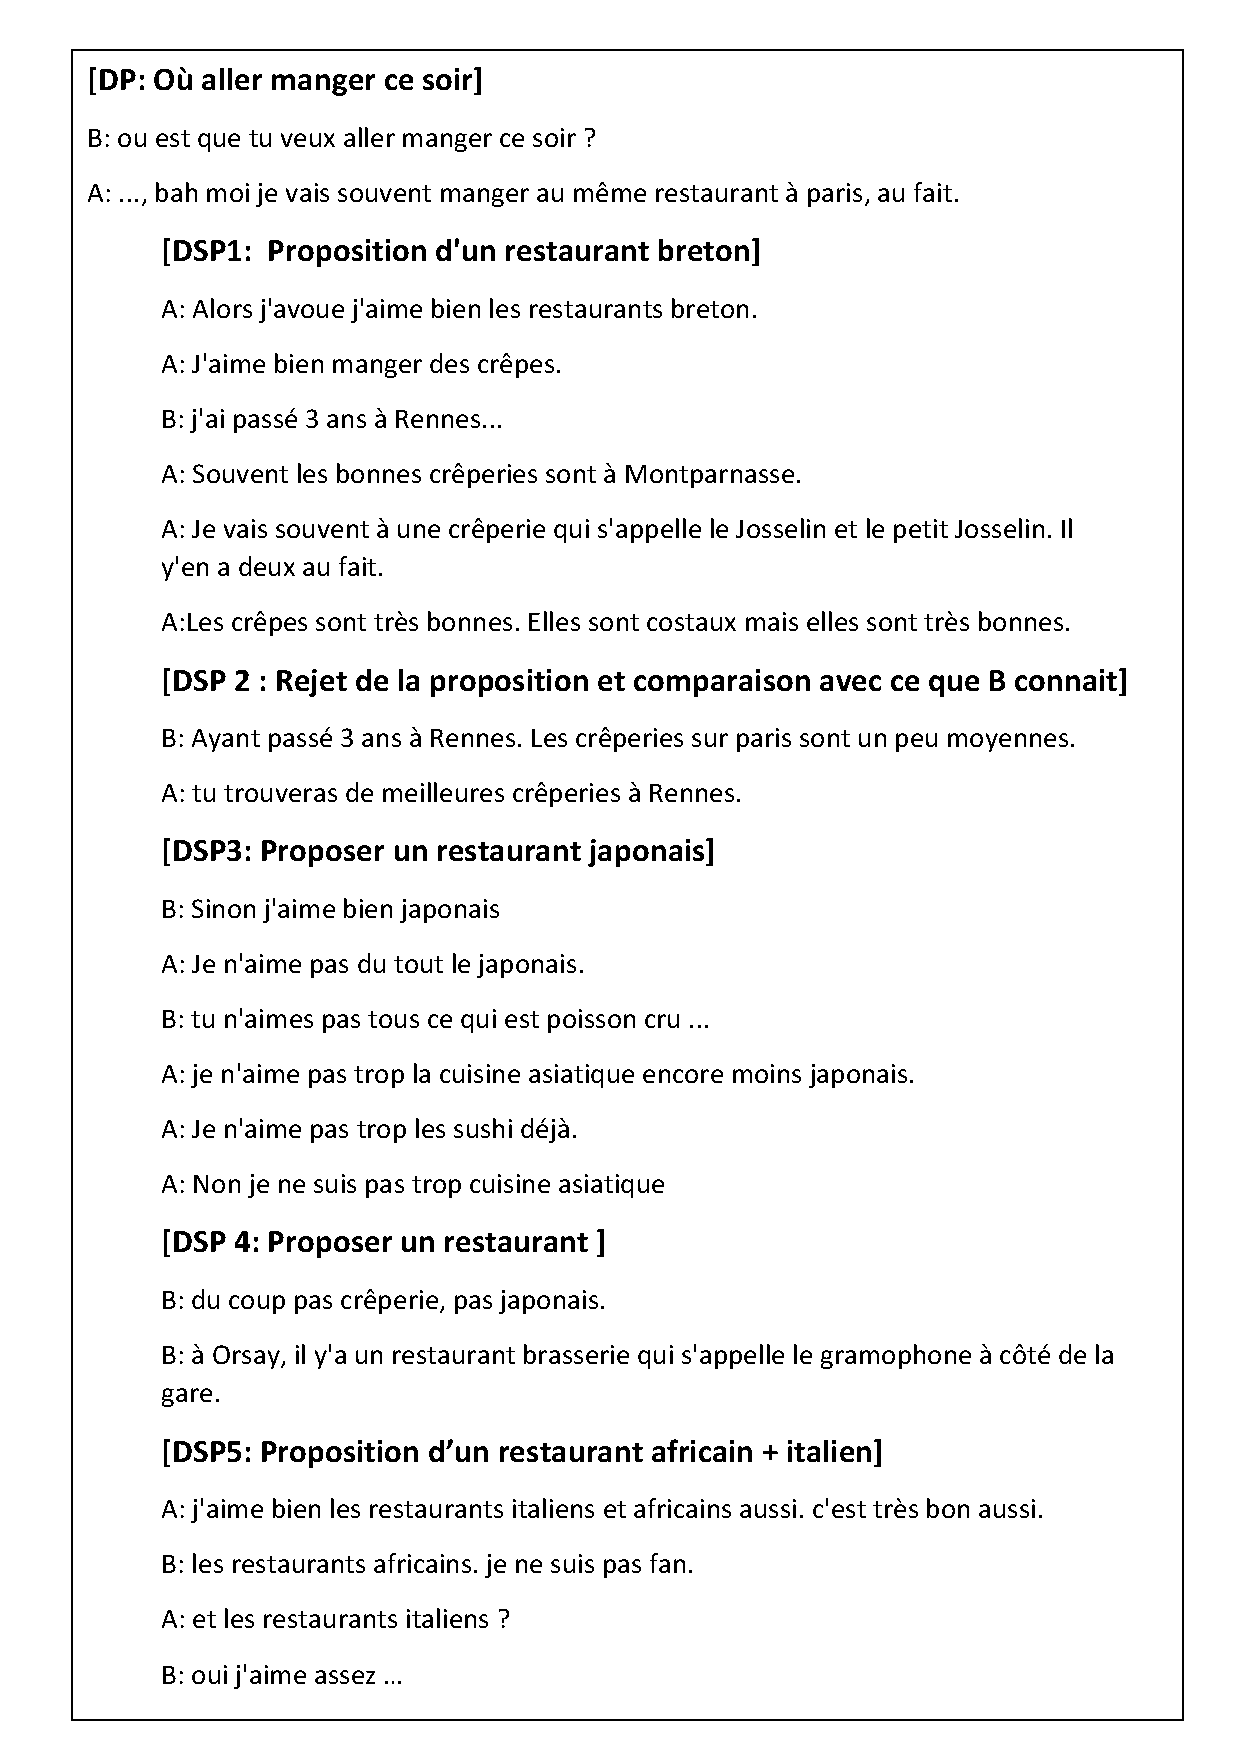
\includegraphics[width=5in]{Figures/dsp_analysis.pdf}
				\caption{\label{fig:conc} Exemple d'une décomposotion en \emph{discourse segment} \emph{DS}}
			\end{figure} 
			 
		\subsection{Résultats de l'analyse}
		
			L'analyse en DSPs nous a révélé un nombre de comportements intéressants tant sur l'aspect structurelle de la négociation que sur les stratégies de négociations déployées par les interlocuteurs. 	
			
			Sur l'aspect structurelle, la décomposition du dialogue en \emph{DS} nous a confirmé que les négociateurs s'intéressaient à différents critères pour le choix d'une option (restaurant dans notre exemple). Ces critères sont négociés simultanément durant la négociation jusqu'a ce que les interlocuteurs trouvent un compromis qui les satisfasse sur les critères jugés importants. 
			Par exemple, dans le premier dialogue, les interlocuteurs se sont plus intéressés à l'ambiance du restaurant et son emplacement pour le choix final. En revanche, dans le second dialogue, les interlocuteurs se sont principalement intéressés aux type et la qualité de la cuisine.
			    
			De plus, Les critères les plus importants sont les premiers à être abordés, et en cas de conflit, d'autre critères sont abordés. 
			Ceci est confirmé par des travaux en négociations automatiques qui mettent en avant l'intérêt de la modalisation multicritères dans les systèmes de négociation. Ce point sera abordé plus en détails en section suivante. 
			 
			 Nous nous sommes aussi intéressé à l'aspect dialogique de la négociation. En effet, notre modèle se basant sur des actes de dialogue, nous avons analysé les différentes informations échangées lors de la négociation. 
			 Nous avons récoltés des informations sur le style linguistique à affecter à nos actes de dialogues.
			 
			 Finalement, nous avons utilisé la structure attentionnelle et intentionnelle afin d'étudier les stratégies de négociation adoptées par les négociateurs. nous avions analyser la corrélation entre différents comportements durant la négociation influencés par la dimension de la dominance.
			 
			 Le résultats obtenus montrent qu'une relation complémentaire de dominance s'installe entre les négociateurs. C'est à dire que dans la situation où un négociateur prend le pouvoir, l'autre parti accepte cette prise de pouvoir et adapte son comportement.
		
			 La prise de pouvoir se manifeste par les stratégies de prise de parole. Le négociateur avec un haut niveau de dominance avait tendance à prendre la parole plus fréquemment, et plus longtemps. Par exemple, en analysant le \emph{DS1} et \emph{DS3}, nous observons que l'interlocuteur \textit{B} prend plus de tours de parole et pour chaque tour, plusieurs actes dialogiques sont énoncés. 
			 %Par conséquent, en moyenne, la
			 
			 
			 De plus, le style linguistique traduit aussi un comportement de dominance, nous avons observé que la personne dominante avait tendance à facilement exprimer ses préférences (\emph{e.g.} voir \emph{DS3}), argumenter ses choix et décisions dans le but de convaincre l'autre. 
			 
			Ces résultats obtenus ont soutenu les comportements de dominance relayé dans les travaux en psychologie sociale et nous ont aidé a orienter la conception de notre modèle de dialogue
			
		
	
	\section{Domaine de négociation}
	\label{domaine}
	
	%	L'interet d'une négociation multi-critères dans la modélisation d'un sujet social
	% voir intro :https://www.ri.cmu.edu/pub_files/pub4/lai_guoming_2008_1/lai_guoming_2008_1.pdf
	%https://link.springer.com/content/pdf/10.1007/s10458-006-9009-y.pdf
	
		La recherche en négociation automatique peut être divisée en deux catégories en ce qui concerne la représentation du domaine: négociation sur un critère et la négociation multi-critères. Cependant, La littérature existante se concentre plus sur la négociation uni critère \cite{lai2008decentralized,lai2004literature}. 
		
		Dans le cadre d'une interaction avec un négociateur humain, la négociation multi-critère est cruciale. En effet, dans un environnement humain, les négociateurs peuvent discuter de plusieurs critères simultanément, ce fait est aussi observé dans l'étude que nous avions effectué dans la section précédente.  Nous avons observé que les négociateurs s'intéressaient à plusieurs critères pour le choix d'un restaurant. Par exemple le type de cuisine, la location ou encore l'ambiance de ce dernier. Ces critères ont soit été abordé simultanément dans la négociation, ou bien un par un. C'est à dire que les négociateurs s'accordaient sur un premier critère avant d'aborder un autre, ou bien discuter des différents critères jusqu'à aboutir a un compromis.
		
		De plus, plusieurs travaux en négociation automatique ont mis en exergue l'apport de la négociation multi-critères. Elle permet d'augmenter la coordination et collaboration durant le processus de négociation afin de rechercher un résultat qui apporte des gains communs pour les deux parties \cite{jonker2007agent,lai2008decentralized,lai2004literature}. 
	
		% 	Pour toutes ces raisons, notre choix s'est porter sur la négociation multi-critère
	
		Les résultats des précédents travaux nous ont motivé à utiliser une représentation multi-critère pour modéliser notre domaine de négociation collaborative. 
		
		\subsection{Représentation formelle des éléments de la négociation }	
		Le but de la négociation est de choisir une \textit{option} $O$ dans l'ensemble des options $\mathcal{O}$ comprenant toutes les options alternatives envisagé pour un sujet de négociation donnée. 
		
		L'évaluation de chaque option repose sur un ensemble de critères $\mathcal{C}$ reflétant les caractéristiques de l'option. Nous définissons l'ensemble $\mathcal{C}$ de $n$ critères, et $C_1,\ldots,C_n$, comme le domaine de valeurs de chaque critère de l'ensemble. 
		Par conséquent, $\mathcal{O}$ peut être défini comme le produit vectoriel de  $C_1\times\ldots\times C_n$ et chaque option $O \in \mathcal{O}$ est un tuple $(v_1,\ldots,v_n)$. 
		
		Par exemple, une négociation collaborative qui porte sur le choix d'un restaurant où dîner peut être modélisé en prenant en compte quatre critères à savoir $\mathcal{C} = \{Cuisine, Prix, Emplacement, Athmosphère, \}$. La table \ref{tab:domain} résume un exemple de domaine de valeurs possible pour chaque critère. Nous faisons l'hypothèse que l'agent connaisse toutes les options pour un domaine donné. Un exemple d'option est $ Anterprima(Italien, coûteux , animé, west side)$. Au total, $638$ options peuvent être généré à partir du domaine présenté dans la table \ref{tab:domain}. 
		\begin{table}[h]
			\centering
			\begin{tabular}{|p{2.25cm}|p{9.25cm}|}
				\hline
				Critère $i $ & Domaine de valeur $C_i$ \\
				\hline
				Cuisine & \{Italien, Français, Japonais, Chinois, Mexicain, Turque, Coréen\} \\
				\hline
				Atmosphère & \{Animé, Calme, Romantique, Familial, Cosy, Moderne\} \\
				\hline
				Prix & \{Coûteux, abordable, a prix bas\} \\
				\hline
				Emplacement & \{West side, East side, Downtown, North side, South side\} \\
				\hline
				
			\end{tabular}
			\caption{Domaine de valeurs pour les critères de choix d'un restaurant} 
			\label{tab:domain}
		\end{table}
		
		
		\subsection{Préférences}
		
			L'agent conversationnel est défini avec un ensemble de préférences formalisé  par un ordre partiel $\prec_i$, défini sur chaque domaine de critères $C_i$. 
					\begin{figure}[!tb] 
						\centering 
						\begin{tabular}{l}
							\subfloat[]{\adjustbox{raise=-5pc}{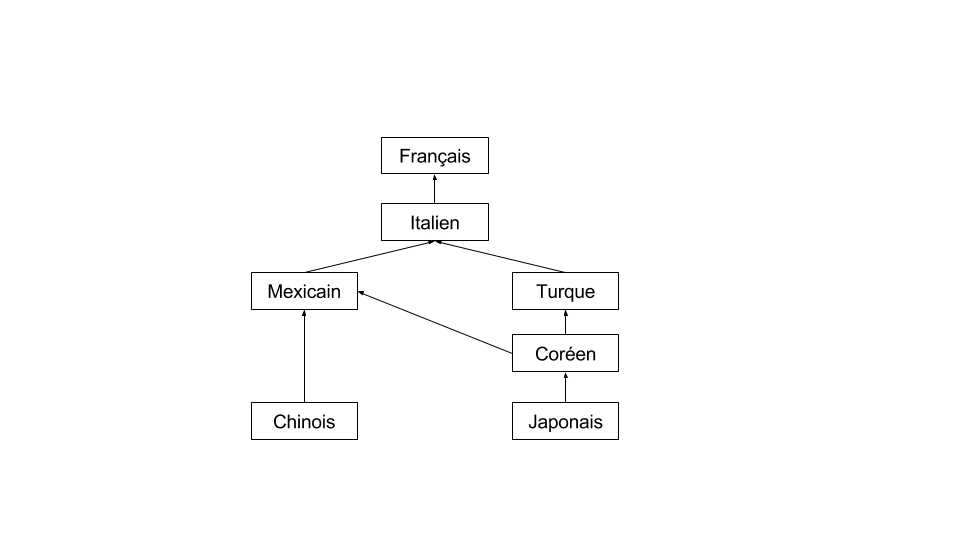
\includegraphics[height=4.8cm]{Figures/cuisine_ex2.png} \label{fig:sub_pref}}}
							\subfloat[]{
								%\input{Figures/Tikz/goldMineState.tex}\label{fig:goldMineState}}  
								\begin{tabular}{|c|c|}
									\hline
									& Critère cuisine \\
									\cline{2-2}
									\parbox[t]{2mm}{\multirow{7}{*}{\rotatebox[origin=c]{90}{\textbf{Préférences}}}} & Japonais $\prec_{cuisine}$ Coréen\\
									\cline{2-2}
									& Chinois $\prec_{cuisine}$ Mexicain\\
									\cline{2-2}
									&  Coréen$\prec_{cuisine}$ Mexicain\\
									\cline{2-2}
									&  Coréen $\prec_{cuisine}$ Turque \\	
									\cline{2-2}
									&  Mexicain$\prec_{cuisine}$ Italien \\
									\cline{2-2}
									&  Turque $\prec_{cuisine}$ Italien\\
									\cline{2-2}
									&  Italien $\prec_{cuisine}$ Français\\	
									\hline								
								\end{tabular}}
							\end{tabular}
							\caption{Exemple de modèle de préférences défini sur le critère cuisine}
							\label{fig:ex_pref}
						\end{figure}
			Nous définissons la relation de préférence comme une relation binaire. Par exemple, $japonais \prec_{cuisine} italien$ signifie que l'agent préfère la cuisine italienne à la cuisine japonaise. Elle est aussi transitive, par exemple, l'agent dispose d'une autre préférence $italien \prec_{cuisine} français$. Nous pouvons donc déduire que l'agent $japonais \prec_{cuisine} français$.
			
			 Ces conditions garantissent que les préférences de l'agent sont cohérentes dans le domaine de la négociation; et la condition de transitivité assure que toutes les valeurs sont comparables. Un exemple de modèle de préférences défini sur le critère de cuisine est présenté dans la figure \ref{fig:ex_pref}.
			
			
			Les préférences étant un aspect essentiel dans la prise de décision durant la négociation, nous avons modélisé une fonction qui représente la valeur d'utilité ou satisfaction pour chaque valeur calculé à partir de l'ensemble des préférences. Donc, pour un critère $i\in \mathcal{C}$, pour une valeur $v\in C_i$, l'agent calcule sa \emph{satisfaction} $sat_{self}(v \prec_i)$ pour cette valeur comme le nombre de valeurs qu'il préfère moins dans l'ordre partiel des préférences $\prec_i$. La valeur est ensuite normalisé dans l'intervalle [0,1]:
			
			\begin{equation}
			sat_{self}(v, \prec_i) =	1 - \left( \frac{|\{v' : v' \neq v \  \wedge \ (v \prec_i v')\}| }{( |C_i| - 1 )}\right)
			\end{equation}
			
			La notion de satisfaction est généralisé pour chaque option $o= (v_1, \ldots, v_n)\in \mathcal{O}$ comme une moyenne des valeurs de satisfactions des différentes valeurs de critères: 
			\footnote{Il existe une grande quantité de travaux  dans le domaine de la prise de décision  qui traitent sur la combinaison de plusieurs critères pour le calcul d'utilité en utilisant par exemple des moyennes pondérées ou des intégrales de Choquet. Nous nous ne intéressons pas dans nos travaux à l'optimisation de la fonction de calcul, pour cette raison nous optons pour une fonction simple d'agrégation de préférences.}
	
			\begin{equation}
			sat_{self}(o, \prec) = \frac{\sum_{i=1}^{n} sat_{self}(v_i, \prec_i) }{n}
			\end{equation}
		
			Un exemple de valeurs de satisfactions calculé à partir de l'ensemble des préférences de l'exemple \ref{fig:ex_pref} est illustré dans la table \ref{tab:sat}
					\begin{table}[h]
						\centering
								{\scriptsize
						\begin{tabular}{ |c|c|c|c|c|c|c|c| }
							\hline				
							valeur & Italien & Français & Japonais & Chinois & Mexicain & Turque & Coréen \\
							\hline
							
							sat(valeur) & 0.83 & 1 & 0.16 & 0.5 & 0.66 & 0.66 & 0.33 \\
							\hline
							
						\end{tabular}}
						\caption{Valeurs de satisfiabilité pour le modèle de préférences défini sur le critère de cuisine}
						\label{tab:sat}
					\end{table}
	
	\subsubsection{Communication}
		Le modèle de communication étant implémenté sur la plateforme \emph{Disco} \cite{rich09}, l'agent communique avec l'utilisateur via des actes de dialogues. Chaque acte de dialogue a un ensemble spécifique d'arguments et est associé à une expression spécifique formulé dans un langage naturel (NL).
		
		La modélisation des actes de dialogue est basée sur les travaux de Sidner \cite{sidner1994artificial} qui avait proposé des actes de dialogues qui permettent à un agent de communiquer dans le contexte de négociation collaborative. Ces actes lui permettent aussi de gérer son état mental en terme d'intention et croyances communiquées durant la négociation. 
		
		Nous avons définis cinq types d'actes de dialogues génériques et deux actes additionnels pour la fin de négociation. Les actes de dialogues sont présentés dans la table \ref{table:utt}. Seule la génération en NL de ces énoncés doit être spécifié pour le domaine de négociation. La valeur /$v$/ dans la table \ref{table:utt} fait référence au format en NL pour exprimer une valeur d'un acte de dialogue.
		Nous utiliserons tout le long de ce manuscrit l'exemple d'une négociation collaborative pour le choix d'un restaurant. 
		
		Chaque type d'acte de dialogue prend un argument qui peut être soit un une valeur de critère  $v \in C_i$, une option $o \in \mathcal{O}$ ou encore critère $i \in \mathcal{C}$. 
		
		En fonction des informations qu'ils communiquent, ces actes de dialogues peuvent être divisé en trois groupes:
		
		\begin{enumerate}
			
			\item \textit{Actes de dialogues informatifs}; ce groupe fait référence aux actes de dialogues utilisés pour échanger des informations sur les préférences respectives des négociateurs, à savoir (\textit{AskValue/AskCriterion} et \textit{StateValue}). 
			Nous avons fait le choix d'attribuer une seule valeur pour les actes informatifs car nous avions observé dans les négociations humain/humain enregistrés que les négociateurs utilisaient généralement une formulation pour exprimer les valeurs qu'ils appréciaient ou non. Par exemple \textit{I (don't)like Chinese restaurants} plutôt qu'une expression avec une comparaison binaire du type \textit{I like Chinese more than French}.
			
			\item \textit{Actes de négociation}; ces actes de dialogues permettent à l'agent de gérer la négociation en exprimant des propositions a son interlocuteur (\textit{Propose}) ou bien de répondre à des propositions exprimées par son interlocuteur. L'agent peut accepter ou rejeter une proposition (\textit{Accept, Reject}). Les valeurs en arguments dans les actes de négociation peuvent être soit des valeurs de critère comme (``Let's go to a Chinese restaurant''), soit des options  (``Let's go to \emph{Chez Francis}''). 
			
			\item \textit{Actes de fin de négociation}; les actes  (\textit{NegotiationSuccess} or \textit{NegotiationFailure}) sont utilisés pour clore une négociation soit par une réussite, soit par un échec. Le choix de l'acte dépend de l'état mental de l'agent. En effet, si une option est acceptée par les deux négociateurs, l'agent exprime alors un \textit{NegotiationSuccess} et termine la négociation. Sinon, si la négociation échoue, alors l'agent exprime un \textit{NegotiationFailure}. Les conditions d'échec d'une négociation sont présentées dans le chapitre suivant. 
			
		\end{enumerate}
		 
		
		
			\begin{table}[t]
					\centering
					\begin{tabular} {|p{3.25cm}|p{4cm}|p{3.25cm}|}
						\hline
						\textbf{Type d'acte de dialogue}  &\textbf{ Génération en NL} & \textbf{Postcondition}\\
						\hline
						StateValue(v) &  I (don't) like /$v$/. & Speaker : $v \in S_i$ \newline Hearer:  \newline $v\in A_i$ is likable, $v\in U_i$ otherwise \\
						\hline
						AskValue(v)& Do you like /$v$/ ? & \multirow{2}{*}{} \\
						
						AskCriterion(i) &  What kind of /$i$/ do you like ? & \\
						\hline
						ProposeOption(o)  & Let's go to /$o$/. & $o \in P$\\
						
						ProposeValue(v) & Let's go to a /$v$/. & $v \in P_i$\\
						\hline
						AcceptOption(o)& Okay, let's go to /$o$/.& $o \in T$ \\
						
						AcceptValue(v) & Okay, let's go to a /$v$/.& $v \in T_i$ \\
						\hline
						RejectOption(o) & I'd rather choose  something else. & $o \in R$\\
						
						RejectValue(v) &  I'd rather choose  something else. & $v \in R_i$ \\
						\hline
						NegotiationSuccess &  We reached an agreement. & \multirow{2}{*}{}\\
						\cline{1-2}
						NegotiationFailure &  Sorry, but I no longer want to discuss this. & \\
						\hline
						% Counter Propose & $(r,p)\in C_i^2 \vee (r,p) \in \mathcal{O}^2 $ & I don't want to go to $r$. Let's rather go to $p$ \\
						% \hline 
						% RejectState & $x \in \mathcal{O} \vee x\in C_i$ &  I don't like /$x$/, let's choose something else. \\
						% \hline
						% AcceptPropose & $o \in \mathcal{O}$ & Okay. Let's go to /$o$/.\\
						% \hline
					\end{tabular}
				
				\caption{\label{table:utt}Liste des actes de dialogues pour le modèle de négociation collaborative.}
			\end{table}
		
			\subsection{Mise à jour des connaissances durant la communication}
			
			Le choix d'un type d'acte de dialogue est le résultat d'un processus décisionnel que nous détaillerons dans le chapitre \ref{chap:dec}. 
			Afin de prendre des décisions pertinentes, l'agent garde en mémoire l'historique des échanges d'informations formulé au cours de la négociation.  En effet, après chaque acte de dialogue échangé, l'agent met à jour son état mental.  
			
			
			Pour chaque critère $i\in\mathcal{C}$, l'agent construit un ensemble $S_i \subseteq C_i$ des préférences sur les valeurs de ce critère qu'il a déjà communiqué. Cela prévient la répétition d'informations échangées précédemment. 
			De plus, l'agent garde en mémoire les préférences communiquées par son interlocuteur. Nous notons les ensembles $A_i\subseteq C_i$ et $U_i\subseteq C_i$, respectivement l'ensemble des valeurs que l'interlocuteur a communiqué comme appréciées (\textit{I like $\ldots$}) et non appréciées  (\textit{I don't like $\ldots$}) à travers l'acte de dialogue \textit{StatePreference}. 
			
			L'agent maintient aussi des informations sur le cours de la négociation. Soient $P_i \subseteq C_i$, $T_i\subseteq C_i$ et $R_i\subseteq C_i$ les ensembles de toutes les valeurs proposées, acceptées et rejetées pour chaque type de critère. 
			De même, nous considérons $P\subseteq \mathcal{O}$, $T\subseteq \mathcal{O}$ et $R\subseteq \mathcal{O}$ les ensembles de toutes les options proposées, acceptées et rejetées au cours de la négociation.
			
			\subsubsection{Préférences de  l'interlocuteur}
				Dans le contexte d'une négociation collaborative, l'agent prend en compte les préférences de son interlocuteur pour prendre des décision. Pour cette raison, l'agent a besoin de collecter des informations sur les préférences de son interlocuteur. En effet, l'agent utilise les ensembles $A_i$ et $U_i$ qui représentent les préférences de l'interlocuteurs collectés lors des interactions, pour calculer une valeur de \emph{satisfaction}  qu'a l'interlocuteur pour toute valeur $v\in C_i$: 
				
					\begin{equation}
					sat_{other}(v)= \left\{\begin{array}{ll}
					1	 & \mathrm{if\ }  c \in A_i\\
					0    & \mathrm{if\ }c \in U_i\\
					0.5	 & \mathrm{otherwise}
					\end{array}\right.
					\end{equation}
					
				Notons que l'agent possède une connaissance partielle des préférences de son interlocuteur. Par conséquent, les préférences sur certaines valeurs peuvent rester inconnues. Dans  le contexte d'une négociation collaborative, ces valeurs sont considérées comme \textit{potentiellement satisfiables}. Par conséquent, nous leur affectons une valeur arbitraire fixée à \textbf{0.5}.
				
	\section{Conclusion}
			Ce chapitre a présenté les différents éléments de notre modèle de négociation collaborative essentiel pour étudier l'impact de la dominance durant la négociation. Nous avons fait le choix de construire un modèle de négociation générique capable de gérer différent sujets de conversation. De plus, nous avions l'objectifs de définir un domaine qui nous permettrait de refléter différents comportements durant la négociation. 
			
			Premièrement, nous avons appuyé notre recherche par une collecte de données où nous avons enregistré des négociations humains/humain qui nous a révélé nombres de comportements qui apparaissent au cours de la négociation. Ces résultats ont été discutées et nous ont permis de guider notre recherche. Entre autres, les résultats obtenus nous ont soutenu dans notre choix de modéliser une négociation  multi-critères.
			Nous avons donc présenté le domaine de négociation multi-critères ainsi que la représentation classique de préférences.
			
			Nous avons ensuite présenté notre modèle de communication. Le modèle proposé permet à l'agent de mener une négociation collaborative. En effet, les actes proposées permettent à l'agent d'une part d'échanger des informations sur les préférences et d'autre part de négocier. 
			
			Ce modèle de négociation collaborative présente une base solide pour construire un modèle de décision qui prend en compte les comportements de pouvoir. Le chapitre suivant présente donc la construction du modèle décisionnel de notre système de négociation. Nous présenterons un algorithme décisionnel capable de refléter différentes stratégies de négociation en fonction du pouvoir que l'agent cherche à exprimer.
					
			
%	Présentation des actes de dialogues avec leurs catégories et conditions d'applicabilité. 
%	\textcolor{red}{Expliquer que note choix d'utterances se basent sur les travaux de Candece Sidner. De plus, l'analyse en DSP nous a révélé que les participants utiliser des doubles utterances dans leur négociation, et ceci de manière réccurente. Ceci traduisait de plus leur stratégies de négociation influncé par des comportements de pouvoir}
	
